\section{Appendix to Section \ref{sec:decentralized}}\label{app:decentralized}

\subsection{Derivation of national welfare}\label{app:nationalwelfare}

Fix a project type \(j \in \{I,B\}\).
National value under independent ownership is
\begin{equation}
    B_j^{N,D}
    =
    C^D(j)
    + \pi_I^D(j)
    + \pi_E^D(j)
    + \xi_j^D,
\end{equation}
whereas national value under approved acquisition is
\begin{equation}
    B_j^{N,A}
    =
    C^M(j)
    + \Pi^M(j)
    + \xi_j^A.
\end{equation}
The merger-attempt indicator is
\begin{equation}
    a_j(q)=\mathbf{1}\{q\Delta_j \ge k\}.
\end{equation}
Hence expected national value generated by a successful project is
\begin{equation}
    B_j^N(q)
    =
    B_j^{N,D}
    +
    a_j(q)
    \left[
        q\bigl(B_j^{N,A}-B_j^{N,D}\bigr)
        -
        \kappa^N k
    \right].
\end{equation}

Conditional on entry with project \(j\), the entrepreneur chooses effort
\begin{equation}
    x_j^*(q)=R_j(q).
\end{equation}
Hence an entrant with fixed cost \(f\) generates expected national welfare
\begin{equation}
    \omega_j^N(f;s,q)
    =
    R_j(q)B_j^N(q)
    -
    \frac{R_j(q)^2}{2}
    -
    f
    -
    \tau s.
\end{equation}
The entrepreneur enters if and only if
\begin{equation}
    f \le c_j(s,q)=s+\frac{R_j(q)^2}{2}.
\end{equation}
Under the uniform distribution on \([0,1]\), aggregate national welfare is therefore
\begin{equation}
    W_j^N(s,q)
    =
    \int_0^{c_j(s,q)}
    \left[
        R_j(q)B_j^N(q)
        -
        \frac{R_j(q)^2}{2}
        -
        f
        -
        \tau s
    \right] df.
\end{equation}
Integrating gives
\begin{equation}
    W_j^N(s,q)
    =
    c_j(s,q)
    \left(
        R_j(q)B_j^N(q)
        -
        \frac{R_j(q)^2}{2}
        -
        \tau s
    \right)
    -
    \frac{c_j(s,q)^2}{2},
\end{equation}
which is the national special case of the planner-specific welfare block used in Section \ref{sec:decentralized}.

\subsection{Proof of Proposition 3}

Fix \(j\) and \(q\), and suppress arguments for notational simplicity. Let
\[
R \equiv R_j(q), \qquad B \equiv B_j^{PM}(q), \qquad A \equiv \frac{R^2}{2}.
\]
By construction, benchmark welfare conditional on project \(j\) is
\[
W_j^{PM}(s,q)=\int_0^{c_j(s,q)}
\left[
RB-\frac{R^2}{2}-f-\tau s
\right]df,
\]
with
\[
c_j(s,q)=s+\frac{R^2}{2}=s+A.
\]
Therefore
\[
W_j^{PM}(s,q)
=
(s+A)(RB-A-\tau s)-\frac{(s+A)^2}{2}.
\]
Expanding,
\[
W_j^{PM}(s,q)
=
-\left(\tau+\frac12\right)s^2
+
\bigl[RB-(\tau+2)A\bigr]s
+
A(RB-A)-\frac{A^2}{2}.
\]
Hence
\[
\frac{\partial W_j^{PM}(s,q)}{\partial s}
=
RB-(\tau+2)A-(2\tau+1)s,
\]
and
\[
\frac{\partial^2 W_j^{PM}(s,q)}{\partial s^2}
=
-(2\tau+1)<0.
\]
Thus \(W_j^{PM}(s,q)\) is strictly concave in \(s\), and the unconstrained maximizer is
\[
s=\frac{RB-(\tau+2)A}{2\tau+1}.
\]
Substituting \(A=R^2/2\) yields
\[
s=\frac{R_j(q)B_j^{PM}(q)-\frac{\tau+2}{2}R_j(q)^2}{2\tau+1}.
\]
Imposing the constraint \(s\ge 0\) gives
\[
s_j^{PM*}(q)
=
\max\left\{
0,\,
\frac{R_j(q)B_j^{PM}(q)-\frac{\tau+2}{2}R_j(q)^2}{2\tau+1}
\right\}.
\]
This proves Proposition 3.

\subsection{Proof of Proposition 4}

Fix a project type \(j\in\{I,B\}\).

For \(q<\bar q_j\equiv k/\Delta_j\), no merger is attempted, so
\[
a_j(q)=0,
\qquad
R_j(q)=\pi_E^D(j),
\qquad
B_j^{PM}(q)=V_j^D.
\]
Therefore
\[
s_j^{PM*}(q)
=
\max\left\{
0,\,
\frac{\pi_E^D(j)V_j^D-\frac{\tau+2}{2}\bigl(\pi_E^D(j)\bigr)^2}{2\tau+1}
\right\},
\]
which is constant in \(q\). This proves part (i).

Now consider an interval on which \(q>\bar q_j\) and the optimal subsidy is interior. On that interval,
a merger is attempted, so
\[
R_j(q)=\pi_E^D(j)+\beta(q\Delta_j-k),
\qquad
R_j'(q)=\beta\Delta_j,
\]
and
\[
B_j^{PM}(q)=V_j^D+q\Omega_j-k,
\qquad
\frac{dB_j^{PM}(q)}{dq}=\Omega_j.
\]
Because the optimum is interior,
\[
s_j^{PM*}(q)
=
\frac{R_j(q)B_j^{PM}(q)-\frac{\tau+2}{2}R_j(q)^2}{2\tau+1}.
\]
Differentiating,
\[
\frac{ds_j^{PM*}(q)}{dq}
=
\frac{
R_j'(q)B_j^{PM}(q)
+
R_j(q)\frac{dB_j^{PM}(q)}{dq}
-
(\tau+2)R_j(q)R_j'(q)
}{2\tau+1}.
\]
Substituting \(R_j'(q)=\beta\Delta_j\) and \(dB_j^{PM}(q)/dq=\Omega_j\) yields
\[
\frac{ds_j^{PM*}(q)}{dq}
=
\frac{
\beta\Delta_j\bigl[B_j^{PM}(q)-(\tau+2)R_j(q)\bigr]
+
R_j(q)\Omega_j
}{2\tau+1},
\]
which proves part (ii).

For part (iii), if
\[
\Omega_j\le 0
\qquad\text{and}\qquad
B_j^{PM}(q)\le (\tau+2)R_j(q),
\]
then both terms in the numerator are weakly negative, since \(\beta\Delta_j>0\) and \(R_j(q)>0\).
Hence
\[
\frac{ds_j^{PM*}(q)}{dq}\le 0.
\]
This proves Proposition 4.

\subsection{Proof of Proposition 5}

Because the subsidy enters private payoffs additively, it does not affect project choice; by
Corollary 1, the entrepreneur chooses
\[
j^*(q)\in\{I,B\}
\]
as characterized in Proposition 1. Therefore the planner chooses the subsidy taking the privately
selected project as given, so
\[
s^{PM*}(q)=s_{j^*(q)}^{PM*}(q).
\]
Using Proposition 1, this yields
\[
s^{PM*}(q)=
\begin{cases}
s_I^{PM*}(q), & q<\hat q,\\[0.3em]
\{s_I^{PM*}(\hat q),\,s_B^{PM*}(\hat q)\}, & q=\hat q,\\[0.3em]
s_B^{PM*}(q), & q>\hat q.
\end{cases}
\]

Now suppose that
\[
B_B^{PM}(\hat q)<\frac{\tau+2}{2}R_B(\hat q).
\]
Define
\[
\Psi_B^{PM}(q)\equiv B_B^{PM}(q)-\frac{\tau+2}{2}R_B(q).
\]
Under Assumptions 1--3, we have \(\hat q\ge \bar q_I>\bar q_B\), so project \(B\) is merger-feasible at
\(q=\hat q\). Hence both \(R_B(q)\) and \(B_B^{PM}(q)\) are continuous on a right neighborhood of \(\hat q\),
and therefore \(\Psi_B^{PM}(q)\) is continuous there as well.

Since \(\Psi_B^{PM}(\hat q)<0\), there exists \(\varepsilon>0\) such that
\[
\Psi_B^{PM}(q)<0
\qquad
\text{for all } q\in(\hat q,\hat q+\varepsilon).
\]
By Proposition 3,
\[
s_B^{PM*}(q)=0
\qquad
\text{for all } q\in(\hat q,\hat q+\varepsilon).
\]
Because \(j^*(q)=B\) for all \(q>\hat q\), it follows that
\[
s^{PM*}(q)=0
\qquad
\text{for all } q\in(\hat q,\hat q+\varepsilon).
\]
This proves Proposition 5.

\subsection{Proof of Proposition 6}

Fix a project type \(j\) and an approval probability \(q\). Let planner-specific successful-project value be
\[
B_j^p(q)=B_j^{PM}(q)+D_j^p(q),
\]
where \(D_j^p(q)\) is the planner-specific incidence adjustment relative to the primitive benchmark.

Using the same concavity argument as in Proposition 3, the planner-\(p\) problem has the unconstrained
maximizer
\[
u_j^p(q)
=
\frac{R_j(q)B_j^p(q)-\frac{\tau+2}{2}R_j(q)^2}{2\tau+1}.
\]
Substituting \(B_j^p(q)=B_j^{PM}(q)+D_j^p(q)\),
\[
u_j^p(q)
=
\frac{R_j(q)B_j^{PM}(q)-\frac{\tau+2}{2}R_j(q)^2}{2\tau+1}
+
\frac{R_j(q)D_j^p(q)}{2\tau+1}.
\]
Define
\[
u_j^{PM}(q)
\equiv
\frac{R_j(q)B_j^{PM}(q)-\frac{\tau+2}{2}R_j(q)^2}{2\tau+1}.
\]
Then
\[
u_j^p(q)=u_j^{PM}(q)+\frac{R_j(q)D_j^p(q)}{2\tau+1}.
\]
Imposing the subsidy constraint \(s\ge 0\) yields
\[
s_j^{p*}(q)
=
\max\left\{
0,\,
u_j^{PM}(q)+\frac{R_j(q)D_j^p(q)}{2\tau+1}
\right\}.
\]
If, in addition, both the primitive benchmark subsidy and the planner-\(p\) subsidy are interior, then
\(u_j^{PM}(q)=s_j^{PM*}(q)\) and \(s_j^{p*}(q)=u_j^p(q)\), so
\[
s_j^{p*}(q)
=
s_j^{PM*}(q)
+
\frac{R_j(q)D_j^p(q)}{2\tau+1}.
\]
This proves Proposition 6.

\subsection{Proof of Corollary 2}

Suppose both local and national optimal subsidies are interior. Then
\[
s_j^{L*}(q)
=
\frac{R_j(q)B_j^L(q)-\frac{\tau+2}{2}R_j(q)^2}{2\tau+1},
\]
and
\[
s_j^{N*}(q)
=
\frac{R_j(q)B_j^N(q)-\frac{\tau+2}{2}R_j(q)^2}{2\tau+1}.
\]
Subtracting,
\[
s_j^{L*}(q)-s_j^{N*}(q)
=
\frac{R_j(q)\bigl(B_j^L(q)-B_j^N(q)\bigr)}{2\tau+1}.
\]
This proves Corollary 2.

\subsection{Proof of Corollary 3}

Because the uniform subsidy does not affect private project choice, the entrepreneur chooses
\(j^*(q)\) as characterized in Proposition 1. Thus both planners evaluate the same privately selected
project at each \(q\).

Suppose both planner-specific optimal subsidies are interior on the relevant range. Applying the
fixed-project interior formula to the privately selected project type,
\[
s^{L*}(q)-s^{N*}(q)
=
s_{j^*(q)}^{L*}(q)-s_{j^*(q)}^{N*}(q)
=
\frac{R_{j^*(q)}(q)\bigl(B_{j^*(q)}^L(q)-B_{j^*(q)}^N(q)\bigr)}{2\tau+1}.
\]
Using the shorthand notation
\[
\bar R(q)\equiv R_{j^*(q)}(q),
\qquad
\bar B^L(q)\equiv B_{j^*(q)}^L(q),
\qquad
\bar B^N(q)\equiv B_{j^*(q)}^N(q),
\]
we obtain
\[
s^{L*}(q)-s^{N*}(q)
=
\frac{\bar R(q)\bigl(\bar B^L(q)-\bar B^N(q)\bigr)}{2\tau+1}.
\]
This proves Corollary 3.

\subsection{A sufficient condition for local over-subsidization of buyout-oriented entry}\label{app:sufficientlocalover}

This appendix gives a simple decomposition under which \(B_B^L(q)>B_B^N(q)\) can arise.

Suppose local value under project \(B\) can be written as
\begin{equation}
    B_B^L(q)
    =
    \widetilde B_B^L(q) + \mu_B P_B(q),
\end{equation}
where \(\widetilde B_B^L(q)\) is the non-transfer component of local value and \(\mu_B P_B(q)\) is the locally retained share of the buyout price paid by an external acquirer.
Let national value be
\begin{equation}
    B_B^N(q)=\widetilde B_B^N(q),
\end{equation}
where the buyout price does not enter because it is a transfer from the national perspective.

Then
\begin{equation}
    B_B^L(q)-B_B^N(q)
    =
    \widetilde B_B^L(q)-\widetilde B_B^N(q)+\mu_B P_B(q).
\end{equation}
Hence a sufficient condition for \(B_B^L(q)>B_B^N(q)\) is
\begin{equation}
    \mu_B P_B(q)
    >
    \widetilde B_B^N(q)-\widetilde B_B^L(q).
\end{equation}
This decomposition clarifies the economic content of Corollary \ref{cor:wedgeequilibrium}:
a local government may over-subsidize buyout-oriented entry when locally retained exit proceeds are large enough relative to the broader competitive and consumer-surplus losses internalized by the national planner.

\subsection{A sufficient condition for local under-subsidization of acquisition-oriented entry}\label{app:sufficientlocalunder}

This appendix gives a mirror-image decomposition under which
\(
B_B^L(q) < B_B^N(q)
\)
can arise even for buyout-oriented projects.

Suppose that, under project \(B\), local value can be written as
\begin{equation}\label{eq:BLunder}
    B_B^L(q)
    =
    \widetilde B_B^L(q)
    + \mu_B P_B(q)
    - D_B(q),
\end{equation}
where \(\widetilde B_B^L(q)\) is the non-transfer local component of value,
\(\mu_B P_B(q)\) is the locally retained share of buyout proceeds,
and \(D_B(q) \ge 0\) captures locally concentrated losses from acquisition, such as the erosion of local competition, employment, ecosystem density, or knowledge retention.

Let national value be
\begin{equation}\label{eq:BNunder}
    B_B^N(q)=\widetilde B_B^N(q),
\end{equation}
where national welfare does not count the buyout payment as a net surplus component because it is a transfer at the aggregate level.

Then
\begin{equation}\label{eq:underdiff}
    B_B^N(q)-B_B^L(q)
    =
    \widetilde B_B^N(q)-\widetilde B_B^L(q)
    - \mu_B P_B(q)
    + D_B(q).
\end{equation}
Hence a sufficient condition for
\(
B_B^L(q) < B_B^N(q)
\)
is
\begin{equation}\label{eq:suffunder}
    D_B(q)
    >
    \widetilde B_B^L(q)
    - \widetilde B_B^N(q)
    + \mu_B P_B(q).
\end{equation}

Equation \eqref{eq:suffunder} clarifies the economic content of local under-subsidization.
Even when part of the buyout gain is retained locally, the local government may still value acquisition-oriented entrepreneurship less than the national planner if locally concentrated losses from acquisition are sufficiently large.
This case is especially relevant when acquisition weakens local competition, reduces the probability that the startup scales independently within the locality, or dissipates local ecosystem spillovers that are not fully offset by retained founder gains.

\subsection{A transfer-augmented calibration with sign reversal}\label{app:signreversalcalibration}

This appendix reports a simple numerical illustration of the sign-reversal case in Corollary \ref{cor:wedgeequilibrium}.
Starting from the benchmark calibration used in the main text, suppose that approved acquisition of the buyout-oriented project carries an additional locally retained buyout-proceeds term of size
\begin{equation}
    \mu_B P_B = 0.70
\end{equation}
inside local approved-acquisition value.
Equivalently, replace
\begin{equation}
    B_B^{L,A}
\end{equation}
by
\begin{equation}
    B_B^{L,A} + 0.70
\end{equation}
while leaving all other primitives at their benchmark values.
This perturbation leaves the private equilibrium thresholds unchanged but raises local valuation of successful buyout-oriented entry sufficiently to reverse the sign of the equilibrium subsidy wedge once project choice switches from type $I$ to type $B$.

Figure \ref{fig:wedge_sign_reversal_appendix} illustrates the resulting wedge.
For $q<\hat q$, the entrepreneur still chooses the independence-oriented project and the wedge remains negative, as in the benchmark calibration.
For $q>\hat q$, however, the additional locally retained buyout proceeds make acquisition-oriented success more valuable locally than nationally, and the wedge becomes positive.
The figure is reported only to illustrate the possibility result in Corollary \ref{cor:wedgeequilibrium}; it is not the baseline calibration used in the main text.

\begin{figure}[t]
\centering
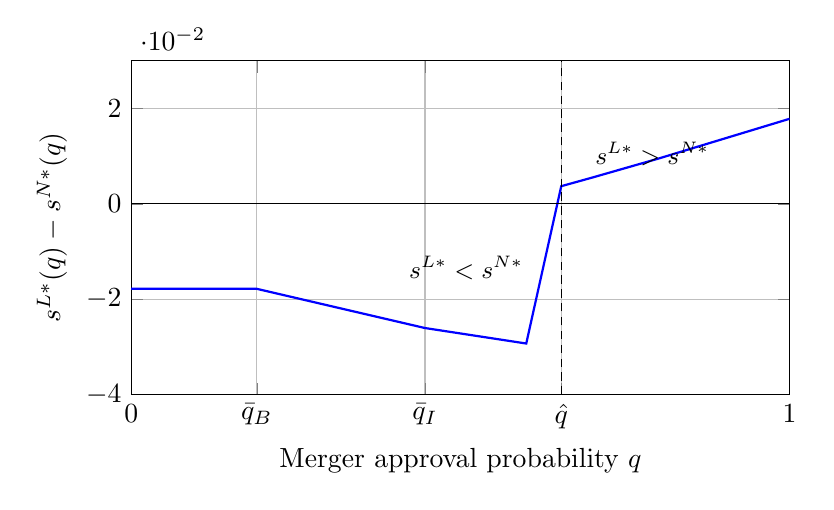
\begin{tikzpicture}
\begin{axis}[
    width=0.82\textwidth,
    height=0.48\textwidth,
    xmin=0, xmax=1,
    ymin=-0.04, ymax=0.03,
    xlabel={Merger approval probability \(q\)},
    ylabel={\(s^{L*}(q)-s^{N*}(q)\)},
    xtick={0,0.1907549041,0.4461335096,0.6531405543,1},
    xticklabels={0,\(\bar q_B\),\(\bar q_I\),\(\hat q\),1},
    ymajorgrids=true,
    xmajorgrids=true
]

\addplot[thick, blue] coordinates {
(0.00,-0.01784)
(0.1907549041,-0.01784)
(0.4461335096,-0.02606)
(0.60,-0.02931)
(0.6531405543,0.00369)
(0.70,0.00549)
(0.80,0.00945)
(1.00,0.01783)
};

\addplot[thin, black] coordinates {(0,0) (1,0)};
\addplot[densely dashed, black] coordinates {(0.6531405543,-0.04) (0.6531405543,0.03)};

\node[anchor=south east] at (axis cs:0.61,-0.018) {\small \(s^{L*}<s^{N*}\)};
\node[anchor=south west] at (axis cs:0.69,0.006) {\small \(s^{L*}>s^{N*}\)};
\end{axis}
\end{tikzpicture}
\caption{Transfer-augmented calibration illustrating sign reversal of the equilibrium subsidy wedge. The benchmark calibration from the main text is modified only by adding a locally retained buyout-proceeds term of size $0.70$ to approved local value for the buyout-oriented project.}
\label{fig:wedge_sign_reversal_appendix}
\end{figure}

\subsection{General distribution of entry costs}\label{app:nationalgeneralG}

Let entry costs be drawn from a continuously differentiable CDF \(G\) with density \(g\).
For project \(j\), the entry cutoff remains
\begin{equation}
    c_j(s,q)=s+\frac{R_j(q)^2}{2}.
\end{equation}
Aggregate national welfare is
\begin{equation}
    W_{j,G}^N(s,q)
    =
    \int_0^{c_j(s,q)}
    \left[
        R_j(q)B_j^N(q)
        -
        \frac{R_j(q)^2}{2}
        -
        f
        -
        \tau s
    \right] dG(f).
\end{equation}
Equivalently,
\begin{equation}
    W_{j,G}^N(s,q)
    =
    \left(
        R_j(q)B_j^N(q)
        -
        \frac{R_j(q)^2}{2}
        -
        \tau s
    \right)
    G(c_j)
    -
    \int_0^{c_j} f\,dG(f).
\end{equation}
Differentiating with respect to \(s\), using \(dc_j/ds=1\), yields the first-order condition
\begin{equation}
    g(c_j)
    \left[
        R_j(q)B_j^N(q)
        -
        R_j(q)^2
        -
        (\tau+1)s
    \right]
    -
    \tau G(c_j)
    =
    0.
\end{equation}
The uniform-distribution national formula in Section \ref{sec:decentralized} is the special case \(G(f)=f\).
